\chapter{Materiais e Métodos}\label{cap:metodologia}

Este capítulo descreverá todo o processo para a criação da metodologia usada. 
Desde a descrição e adaptação do conjunto de dados utilizado, cobrindo as escolhas dos modelos de classificação até a forma de avaliação dos resultados, 
além das tecnologias utilizadas em cada passo.

Apesar de ser possível classificar a situação de alagamento de uma rua em diferentes níveis, para o problema de classificação descrito, 
as diferentes situações foram simplificadas para um problema binário, onde o objetivo é definir se a quantidade de água na rua permite o trânsito de veículos normalmente (classe 0), 
ou a quantidade é o suficiente para impactar o trânsito (classe 1).

\section{Conjunto de dados}\label{sec:dataset}

% explicar por que fiz a escolha por câmeras

O conjunto de dados consiste em imagens de 77 câmeras diferentes da cidade do Rio de Janeiro, capturadas pelo sistema de câmeras do \Acrfull{cor}. 
Neste conjunto, cada câmera possui 30 imagens para cada uma das classes deste problema de classificação binário. 
Ou seja, o conjunto de dados é formado por 60 imagens de cada câmera, totalizando 4620 imagens. 
Do total de 77 câmeras, 60 foram escolhidas para compôr o conjunto de treino e 17 câmeras para validação, ou seja 78\% das câmeras compõem o conjunto de treino e 22\% o conjunto de validação.

Este trabalho frequentemente se refere ao conjunto de dados usado pelo número de câmeras, em vez de descrever diretamente o número de imagens.
Isso é feito propositalmente, visto que foi decidido não utilizar imagens da mesma câmera em treino e em validação, para evitar qualquer tipo de viés em sua validação.
Portanto, cada câmera do conjunto de dados pertence somente ao conjunto de treino ou o conjunto de validação.

Como as imagens foram capturadas em uma cidade movimentada durante o período de chuvas, uma variedade de imagens foi utilizada para o treinamento, 
desde ruas vazias em um dia ensolarado até tráfego intenso em dias chuvosos durante a noite.
Devido a chuvas extremamente fortes, algumas lentes de câmeras estavam muito molhadas para distinguir o que era exibido. Essas imagens não foram incluídas no conjunto de dados.

Ao longo do ano, foram captadas imagens de 472 câmeras distintas, com diferentes proporções de imagens de cada classe para cada câmera. 
Dessa forma, para criar um conjunto de dados balanceado, 
foram escolhidas as câmeras com quantidade suficiente de imagens de ambas as classes para que todas as câmeras do conjunto de dados tenham a mesma quantidade de imagens.

% -----------------------
\subsection{Captação de imagens}

%\textit{\textbf{André: estações de chuva} é algum nome técnico, ou você queria dizer dias de chuvas ou épocas de chuvas?  Ainda você só quer chuvas intensas. Isso parece pela forma como escreveu, mas não fica claro! Explique melhor!} 

As imagens foram captadas ao longo de 2023 em diferentes condições de iluminação e épocas de chuva, com diferentes intensidades de chuva. 
Foi necessário captar tais imagens de maneira eficiente e inteligente, visto que o sistema de câmeras do COR é composto por milhares de câmeras, 
tornando custoso o monitoramento de todas elas, e que as chuvas, apesar de intensas, são imprevisíveis: poderiam cair a qualquer hora, durar intervalos de tempo muito variados.

O sistema de captação foi desenvolvido em Python \cite{van1995python}, utilizando a API do Waze para receber notificações de possíveis situações de alagamento. A biblioteca OpenCV \cite{itseez2015opencv} foi utilizada para a captar as imagens e a API do Google Cloud para upload e armazenamento.
Foram utilizados alertas do aplicativo Waze sobre alagamento de ruas e notificações do próprio sistema do COR para definir quais ruas da cidade do Rio de Janeiro estavam alagadas e assim, começar a captação de imagens dessas ruas. 
%Pois o objetivo da saída binaria é a resposta (sim  ou não) a pergunta: a quantidade de água na rua permite o trânsito de veículos normalmente? 


% -----------------------
\subsection{Análise de imagens}
Para a classificação das imagens, foi criada uma aplicação web baseada em Flask e utilizando MongoDB como banco de dados. 
As imagens já estavam separadas em seis (6) níveis definidos pelo próprio COR. Estes níveis, em ordem crescente de severidade, são: Normal; Poça; Lâmina; Alagamento; Transbordo; e Bolsão. 

%\textit{Você poderia por em exemplo de cada uma em uma tamanho maior queque vem usando, pois eles estão pesando na compilação por serem enormes, nas no texto você as esta colocando pequenas. }

Para simplificar, tendo em vista que não há um limite claramente definido entre cada uma dessas classificações, as classes 'Normal' e 'Poça' foram definidas como classe 0, 
visto que não há impacto no trânsito de veículos. À partir do surgimento de lâminas d'água, 
o trânsito de veículos começa a ser afetado visto que estes devem diminuir sua velocidade para evitar derrapagem \cite{michelinaquaplaning} então, a partir do nível3 'Lâmina', 
as classes mais severas foram definidas como classe 1.

A Figura \ref{fig:class0_1}, mostra uma importante avenida na zona sul do Rio de Janeiro, no entorno da Lagoa Rodrigo de Freitas. 
A Av. Epitácio Pessos na altura da Rua Maria Quitéria, no lado desta lagoa próximo ao bairro de Ipanema. 
A Figura \ref{fig:class0_2}, mostra a rua Jardim Botanico, no cruzamento coma rua Pacheco Leão, no bairro Jardim Botanico.
Estas figuras são exemplos de vias classificadas como \textbf{não alagadas}, ou classe 0. 
Quando há água na via, mas ela não impede o tráfego de veículos, decidiu-se que tais situações não seriam classificadas como \textit{alagamento}.

\begin{figure}[htb]
\centerline{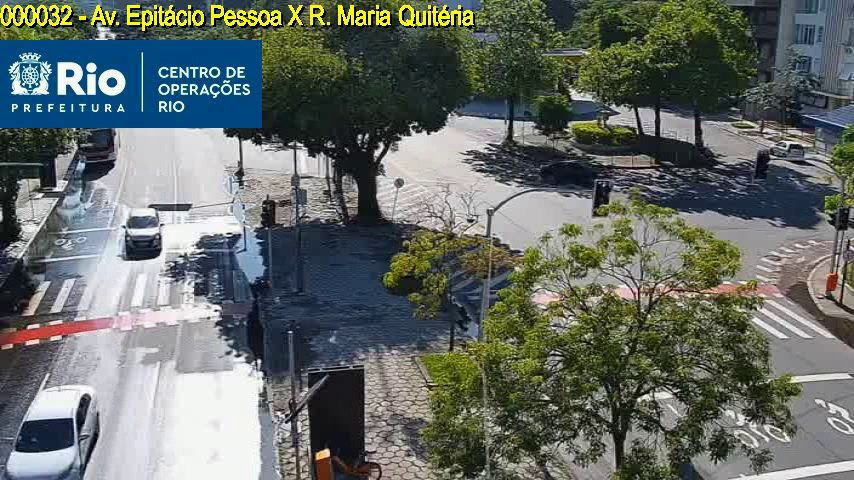
\includegraphics[width=0.8\linewidth]{images/0/CODE32 2023-02-22 08-15-04-6.jpg}}
\caption{Via completamente seca, rotulada como classe 0}
\label{fig:class0_1}
\end{figure}

\begin{figure}[htb]
\centerline{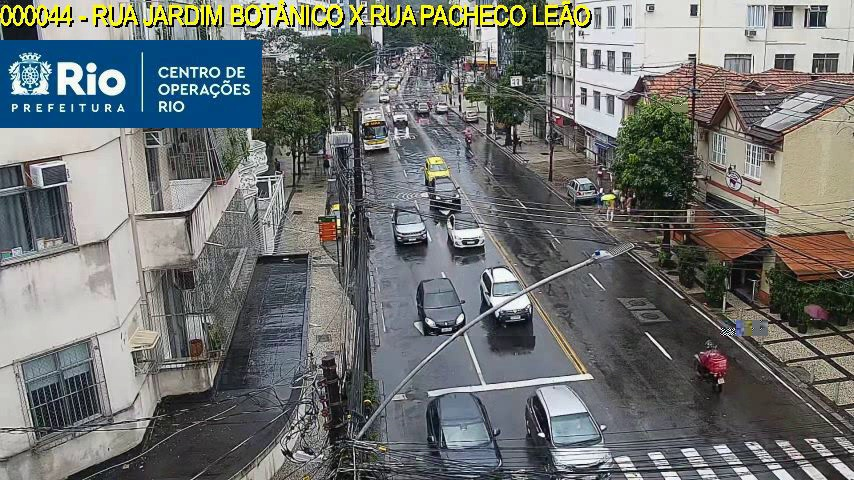
\includegraphics[width=0.8\linewidth]{images/0/CODE44 2023-08-20 13-30-31-6.jpg}}
\caption{Rua molhada, ainda rotulada como classe 0}
\label{fig:class0_2}
\end{figure}

Por outro lado, a Fig. \ref{fig:class1_1} e a Fig. \ref{fig:class1_2} mostram capturas de vias classificadas como \textbf{alagadas}, ou classe 1. 
Em ambas as imagens, é possível ver água cobrindo bastante a rua, dificultando ou impossibilitando a passagem de veículos. 
A Fig. \ref{fig:class1_1} é uma cena capturada pela câmera localizada na zona sul do Rio de Janeiro, no entorno da Lagoa Rodrigo de Freitas. 
A Av. Borges de Medeiros em seu cruzamneto com a Rua Saturnino de Brito, no lado desta lagoa próximo ao bairro Jardim Botânico
A Fig. \ref{fig:class1_1} é o exemplo de uma rua (na zona norte da cidade) parcialmente alagada, dificultante o transito dos veículos onde as calçadas ainda podem ser identificadas. A Fig. \ref{fig:class1_2} é o exemplo de uma rua (da zona sul), sem distinção de calçada ou rua, completamente alagada. Essas situações constituem a classe \textit{alagamento}. 

\begin{figure}[htb]
\centerline{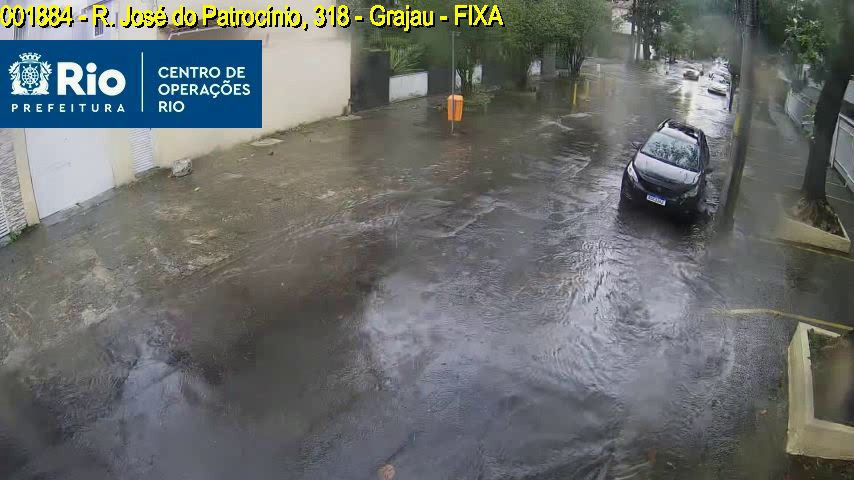
\includegraphics[width=0.8\linewidth]{images/1/CODE1884 2023-08-20 12-56-29-9.jpg}}
\caption{Rua parcialmente alagada (classe 1).}
\label{fig:class1_1}
\end{figure}

\begin{figure}[htb]
\centerline{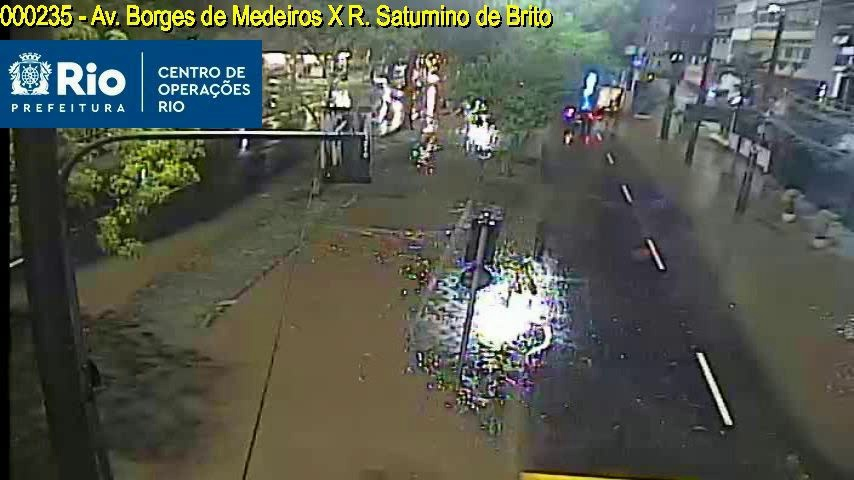
\includegraphics[width=0.8\linewidth]{images/1/CODE235 2023-02-07 20-11-08-9.jpg}}
\caption{Avenida totalmente alagada (classe 1).}
\label{fig:class1_2}
\end{figure}

A Figura \ref{fig:totalcount} mostra um histograma indicando a quantidade de imagens (eixo vertical) de cada classe por cada câmera (eixo horizontal), 
que consiste no conjunto de dados original capturado sem balanceamento das classes. 
As imagens de cada classe correspondem as cores, ou seja se identificam em \textbf{alagadas} ou \textbf{não alagadas} de acordo com as cores (azul ou vermelho) de parte das linhas das câmeras mostradas no eixo horizontal do histograma de distribuição. 
Pode-se observar que algumas câmeras possuem muito mais imagens que a outras, provavelmente por ter ocorrido mais chuvas nas regiões onde estas estão localizadas. 
%Ou seja, estarem em regiões (geográficas) onde há maior distribuição de chuvas na cidade do Rio de Janeiro. 
Assim, a criação de um conjunto de dados sem uma análise prévia da representatividade de cada câmera no conjunto possivelmente criaria um viés em qualquer modelo treinado neste conjunto.

\begin{figure}[htb]
\centerline{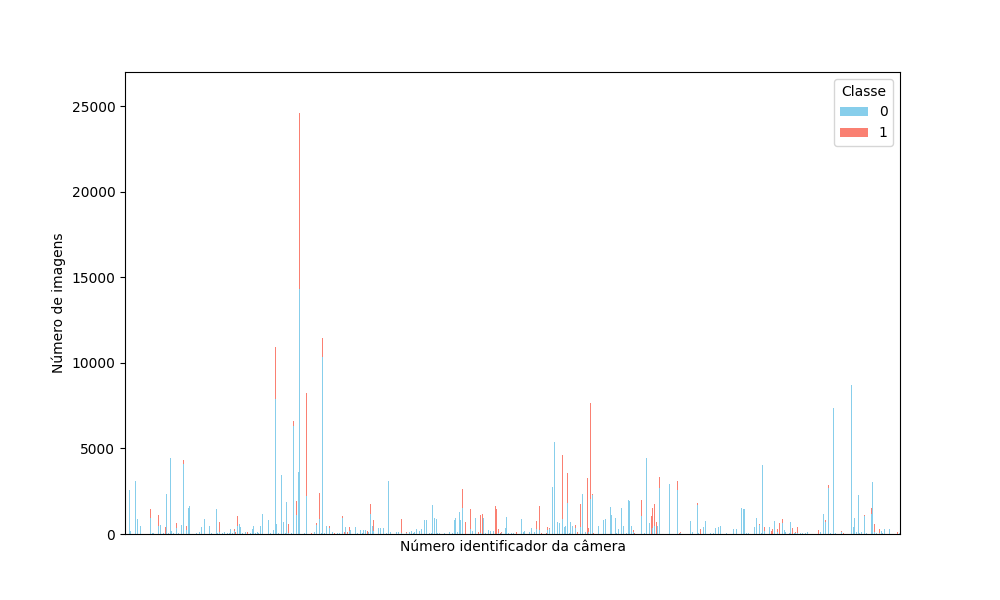
\includegraphics[width=1\linewidth]{images/totalcount_code.png}}
\caption{Histograma de cada classe por câmera disponível.}
\label{fig:totalcount}
\end{figure}

Diminuindo o limite do eixo vertical, se torna mais claro a quantidade de imagens das demais câmeras, como pode ser visto na Figura \ref{fig:totalcountzoom}. A figura indica a quantidade de imagens de cada classe em cada câmera, com eixo vertical
limitado. Assim se identifica que do total de 472 câmeras, 330 delas possuem menos de 500 imagens registradas de ambas as classes, ou 69,9\% delas. Esses dados também não levam em conta a proporção de cada classe no total de imagens em cada câmera.

\begin{figure}[htb]
\centerline{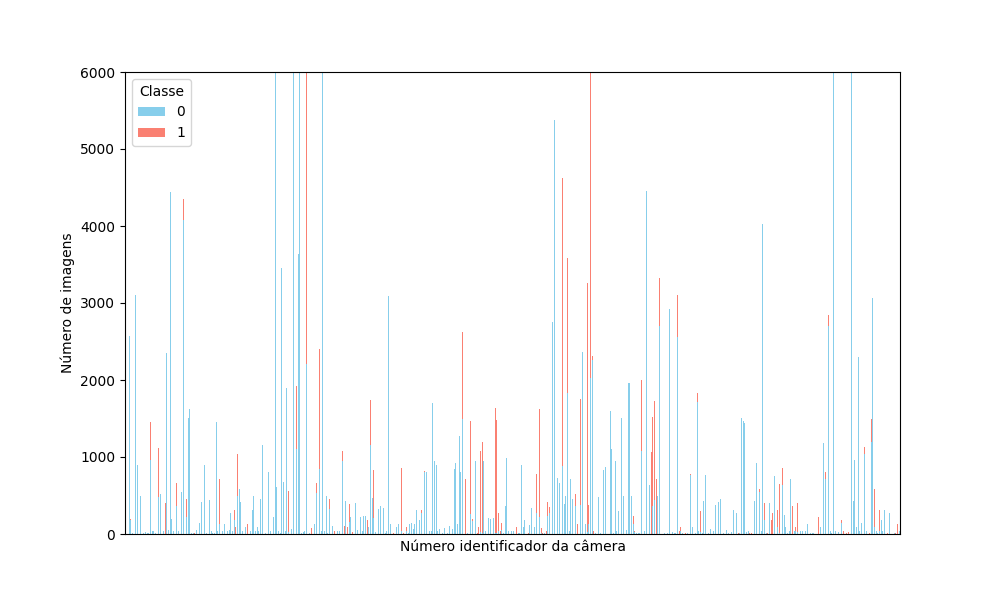
\includegraphics[width=1\linewidth]{images/totalcountzoom_code.png}}
\caption{Histograma com eixo vertical limitado.}
\label{fig:totalcountzoom}
\end{figure}

% \textbf{FAZER UM HISTOGRAMA COM BUCKETS DE QUANTIDADES DE IMAGENS}
% \textbf{SEPARAR POR CLASSES ORIGINAIS (normal, poça, etc}

Diante do exposto, foi necessário considerar qual a quantidade de imagens de cada classe por câmera deve ser considerada para criar um conjunto de dados balanceado e diverso em sua representatividade de câmeras de lugares diferentes. 
Para isso, foi analisada a quantidade de câmeras que possui  um determinado número mínimo de imagens para cada classe, permitindo saber quantas imagens e qual seria a variedade de um conjunto de dados balanceado formado com as imagens captadas e classificadas.

A Figura \ref{fig:balancedcodes} mostra a quantidade de câmeras para a condição descrita. 
Inicialmente, foi julgado que 10 imagens de cada classe por câmeras formaria um conjunto de dados com relativamente poucas imagens levando em consideração as outras possíveis quantidades de imagens por câmera, compondo um conjunto de dados de 1800 imagens, visto que há 90 câmeras com pelo menos 10 imagens de cada classe. 
Um conjunto de dados com 50 imagens de cada classe forneceria 60 câmeras, para um total de 6000 imagens, entretanto, o conjunto de dados ficaria muito maior e com menor variedade de câmeras que usar, por exemplo, o valor escolhido de 30 imagens por câmeras, que teria 77 câmeras. 

\begin{figure}[htb]
\centerline{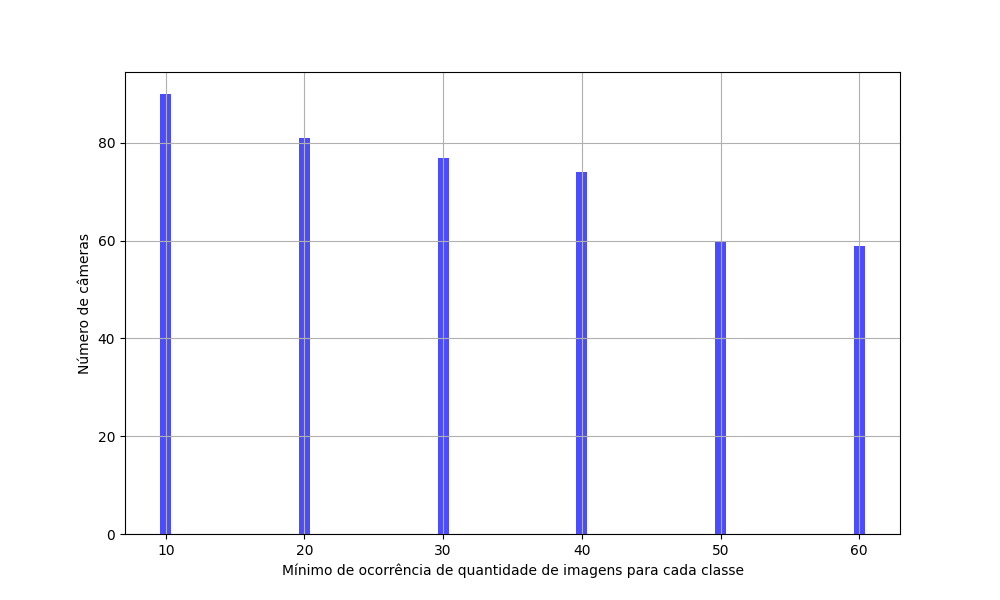
\includegraphics[width=1\linewidth]{images/balancedcodes.png}}
\caption{Quantidade de câmeras com um número mínimo de imagens de cada classe.}
\label{fig:balancedcodes}
\end{figure}

Ao final da avaliação dos modelos de \acrshort{cnn}s, uma reavaliação do número de imagens por câmeras é refeito para tomar uma decisão certa sobre a melhor quantidade de imagens por câmeras, 
e se essa mudança acarretaria melhora nos índices usados para avaliação do modelo, como é apresentado na seção \ref{sec:cameraquantity}.
% -----------------------
\subsection{Pré Processamento}\label{subsec:datapreprocessing}

Diversas etapas de pré-processamento foram aplicadas para melhorar a qualidade das imagens no conjunto de dados.

Primeiramente, uma máscara foi aplicada para remover o logotipo do \acrshort{cor} (ou seja, a região superior esquerda com os brasão da cidade e palavras brancas sobre um fundo azul) das imagens para evitar que o logotipo enviesasse o processo de aprendizado do modelo. Isso foi feito zerando a região da imagem onde o logotipo do COR está localizado, já que sua posição é estática. Como o logotipo está presente em todos os quadros, não foi possível recriar a região apagada com quadros intermediários.

Segundo, como algumas imagens podem apresentar brilho excessivo, os canais de imagem $RGB$ originais foram convertidos para o espaço de cor $YC_rC_b$ para permitir o ajuste no canal \textit{Y}, 
reduzindo o brilho da imagem. Essa transformação no canal \textit{Y} foi feita multiplicando os valores de pixel no canal \textit{Y} por um fator de brilho, 
um número decimal positivo mas menor que 1, com um valor inicial de 0,5. 
Então, cada informação de pixel $YC_rC_b$ é convertida de volta para  \textit{RGB}, para ser mostrada nas telas do computador colorida como originalmente. 
Entretanto, outros valores de fator de brilho (FB) foram avaliados posteriormente na seção \ref{sec:bestmodel}.
As Figuras \ref{fig:samplebright} e \ref{fig:samplebright_half} mostram a mesma cena de um local onde o FB foi aplicado. 
É possível notar a diferença na intensidade do brilho da cena após a alteração no canal \textit{Y}.

\begin{figure}[htb]
    \centerline{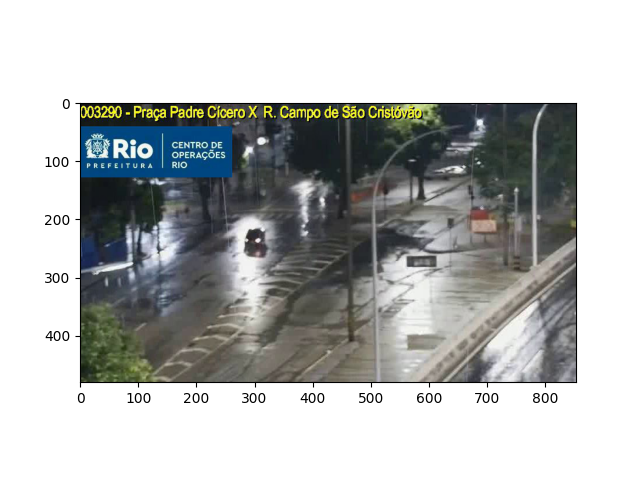
\includegraphics[width=1\linewidth]{images/metodologia/samplebright.png}}
    \caption{Exemplo de região sem alteração no canal \textit{Y}.}
    \label{fig:samplebright}
\end{figure}
\begin{figure}[htb]
    \centerline{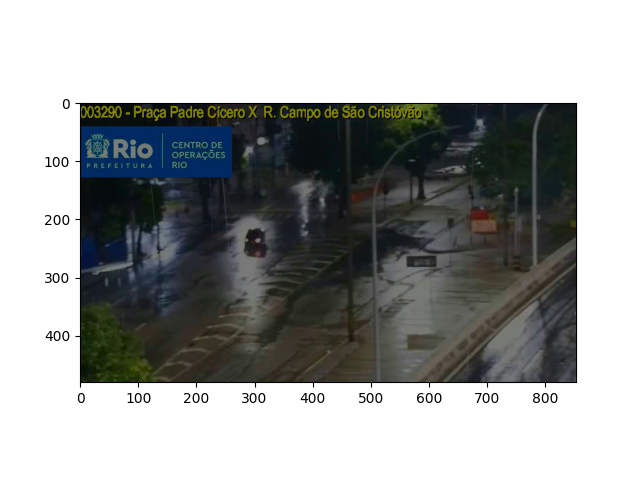
\includegraphics[width=1\linewidth]{images/metodologia/samplebright_half.png}}
    \caption{Exemplo de mesma região com 50\% do valor original de \textit{Y}.}
    \label{fig:samplebright_half}
\end{figure}

%\textbf{Sim precisa fazer isso. Veja que  esse processamento se chama de unsharp masking na literatura , por exemplo LIM, Gonzales, Sonka, etc . E deveria estar na seção de metodologia}

%\textbf{André. isso que fala no inicio do próximo paragrafo deveria ficar em um dos capítulos iniciais, veja que perguntei isto, em relação ao tipo de câmera. Em dissertações você deve é pode ser prolixo, isso não é artigo com máximo de paginas fixas!  Aqui tem que se proteger do membro da banca ler correndo e nem notar algo importante como isso que aqui descreve} 

Para introduzir mais variedade às imagens no treinamento, em seguida foi aplicada uma inversão horizontal aleatória foi aplicada com uma probabilidade de 50\% nos dados de entrada.
Em outras palavras, cada imagem da divisão de treinamento tem 50\% de chance de ser invertida horizontalmente ou não.

Além disso, transformações padrões de redimensionamento, corte e normalização de intensidades são usadas para preparar as imagens para cada modelo $CNN$. 
É aplicado aos dados inicialmente um processo de redimensionamento para transformar cada quadro ajustado ao tamanho esperado de cada modelo,
onde as imagens com dimensão 854 x 480 pixels são redimensionadas para 256 x 256 pixels. 
Então eles são submetidos a um corte de dimensão 224 x 224 pixels de mesmo centro da imagem.
Com exceção do \textit{Inception}, que redimensiona para 342 x 342 pixels e realiza um corte central de 299 x 299 pixels.
Os valores do conteúdo de cada pixel são redimensionados para estarem no intervalo [0,1]. 

%\textit{Andre(não entendi nada do que foi feito pelo falado no próximo paragrafo) RE ESCREVE}

Finalmente, todo o conjunto de dados foi normalizado pela média e desvio padrão específicos de cada modelo:
Todos os modelos avaliados têm a mesma matriz média de (0,485 ; 0,456 ; 0,406) e matriz de desvio padrão de (0,229 ; 0,224 ; 0,225) para cada canal $RGB$, usados para normalizar a imagem. 
%Da mesma forma, eles também compartilham o mesmo tamanho de imagem de 256$\times$256. Com exceção do InceptionV3, que tem tamanho de imagem de 342$\times$342.
% ----------------------------------------------------------
\section{Modelos de classificação}\label{sec:methodology_models}

Com base na nos trabalhos da literatura sobre alagamento urbano anteriormente apresentados, os modelos MobileNetV2 \cite{mobilenetv2}, VGG19 \cite{vgg}, InceptionV3 \cite{inception} e DenseNet \cite{densenet} foram avaliados.
Além disso, a arquitetura de \acrfull{vit}\cite{vit} foi incluída. Essa adição foi feita porque vários modelos de classificação de imagens de alto desempenho são baseados em arquiteturas $Visual$ $Transformers$, como $ViT-Huge$ usado no conjunto de dados CIFAR-10 \cite{dosovitskiy2021image} e $ViT-Large$ no conjunto de dados STL-10 \cite{gesmundo2022continual, kabir2023reduction}.

Todos os modelos foram treinados em 50 épocas, onde o \textit{Early Stopping} foi empregado com uma restrição de 10 épocas e decaimento da taxa de aprendizagem de 0,1. Três diferentes taxas de aprendizagem foram aplicadas em todos os modelos, visto que as diferentes complexidades dos modelos podem resultar em diferentes taxas de aprendizagem ótimas. O \acrfull{sgd} foi usado como otimizador inicialmente, entretanto, outros otimizadores foram testados após a avaliações dos modelos, como pode ser visto na seção \ref{sec:optimizer}.

A transferência de aprendizado foi aplicada a todos os modelos, inicializando-os com os pesos padrões do IMAGENET. Isso foi feito para utilizar os pesos aprendidos anteriormente para auxiliar no aprendizado dos pesos das novas classes \cite{kolesnikov2020big}. Posteriormente, a última camada totalmente conectada foi modificada para ter apenas duas saídas, se adequando ao problema de classificação binária.
% ----------------------------------------------------------
\section{Avaliação dos modelos}

Para avaliar o desempenho dos cinco modelos com diferentes taxas de aprendizagem, inicialmente foi utilizado a acurácia para distinguir o melhor modelo. 
Após a identificação do melhor modelo, a precisão e revocação também foi utilizada para melhor entender seu desempenho. 

Como o conjunto de dados está completamente balanceado, conforme mencionado na Seção \ref{sec:dataset}, com ambas as classes igualmente representativas, esses avaliadores fornecem um cenário adequado para compreensão dos resultados. Adicionalmente, todas as câmeras possuem o mesmo número de imagens, garantindo assim uma representação equilibrada entre as fontes de dados e suas distribuições pela cidade.

Para calcular a acurácia, precisão e revocação, inicialmente foram obtidos os seguintes valores: 
Verdadeiros Positivos (TP), que correspondem ao número de rótulos positivos classificados corretamente pelo modelo; 
Verdadeiros Negativos (TN), que representam os rótulos negativos classificados corretamente; 
Falsos Positivos (FP), que são os rótulos positivos classificados incorretamente; 
e Falsos Negativos (FN), que indicam o número de rótulos negativos classificados de forma incorreta.

O primeiro índice de avaliação selecionada para análise foi a acurácia, 
pois ela fornece uma visão geral da capacidade do modelo em classificar corretamente os exemplos em um conjunto de dados balanceado. 
%Como o objetivo inicial deste estudo é representar com precisão a situação de inundação nas ruas, a precisão e a revocação também foram escolhidas como métricas apropriadas para complementar a análise.

A acurácia pode ser calculada pela seguinte fórmula:
\begin{equation}
    \label{eqn:accuracy}
    Acuracia = \frac{TP+TN}{TP+TN+FP+FN}
\end{equation}

O índice de avaliação de precisão indica a porcentagem de imagens classificadas como positivas que realmente pertencem à classe positiva \cite{FAWCETT2006861}. 
É especialmente relevante para aumentar a confiabilidade do modelo na identificação correta da situação de inundação.

%A precisão é um indicativo da proporção de classificações positivas corretas em relação ao total de predições positivas, e é uma medida importante em contextos onde a minimização de falsos positivos é desejável.%
A Equação \ref{eqn:precision} formaliza o cálculo da precisão:
\begin{equation}
    \label{eqn:precision}
    Precisao = \frac{TP}{TP+FP}
\end{equation}

Além disso, a revocação pode ser empregada como um avaliador final para calcular a taxa de imagens positivas classificadas corretamente \cite{MurphyProbabilistic}. 
Ela é útil para garantir que o menor número possível de situações de inundação seja classificado incorretamente. A revocação mede a capacidade do modelo de identificar corretamente todas as instâncias relevantes.
A equação a seguir define o cálculo da revocação:
\begin{equation}
    \label{eqn:recall}
    Revocacao = \frac{TP}{TP+FN}
\end{equation}

O próximo capitulo apresenta os resultados obtidos. 